\begin{TP}[\MotDefinition{Performance d'un algorithme}{}]

\begin{enumerate}
\item Recopier et compléter l'algorithme suivant pour qu'il calcule $\pgcd(a;b)$.
 
E($x$) signifie la partie entière du nombre $x$.
 
Comment s'appelle-t-il ?

\vspace{-.5\baselineskip}

\begin{center}
  \begin{minipage}{.60\linewidth}
    \begin{algorithme}
      \BlocVariables \DeclareVar{$a$, $b$, $q$, $r$}{\emph{entiers
          naturels}}{} \BlocEntrees \Saisir{$a$, $b$}
      \DonnerValeur{$q$}{$\text{\normalfont
          E}\left(\dfrac{a}{b}\right)$}\vspace{3pt}
      \DonnerValeur{$r$}{$a-bq$} \BlocTraitements
      \TantQue{\dots}{%$r\neq0$
        \DonnerValeur{\dots}{$b$}%$a$
        \DonnerValeur{\dots}{$r$}%$b$
        \DonnerValeur{$q$}{\dots}%$\text{\normalfont E}\left(\dfrac{a}{b}\right)$\vspace{3pt}
        \DonnerValeur{$r$}{\dots}%$a-bq$
      } \BlocAffichage \AfficherVar{\dots}%$b$
    \end{algorithme}
  \end{minipage}
\end{center}

\vspace{-.5\baselineskip}

\item On saisit $a=391$ et $b=221$.
\begin{enumerate}
\item Remplir ce tableau, en calculant à la main les différentes
étapes du programme :

\begin{center}
\renewcommand*\tabularxcolumn[1]{>{\centering\arraybackslash}m{#1}}
\begin{Ctableau}{0.8\linewidth}{5}{c}
\hline
 & $a$ & $b$ & $q$ & $r$\\
\hline
Étape 0 & 391 & 221 & 1 & 170\\
\hline
Étape 1 & & & &  \\
\hline
Étape 2 & & & &  \\
\hline
Étape 3 & & & &  \\
\hline
\end{Ctableau}
\end{center}
\item Rentrer cet algorithme dans la calculatrice et vérifier le
  résultat trouvé.
\end{enumerate}
% \end{enumerate}
% \begin{enumerate}\setcounter{enumi}{2}
\item Modifier cet algorithme pour qu'il affiche le nombre d'étapes
  nécessaires pour calculer $\pgcd(a;b)$. Combien d'étapes sont
  nécessaires pour calculer le PGCD de \enskip $a=\nombre{87
    724}$\enskip et\enskip $b=\nombre{23296}$ ?
\item On voudrait connaître le nombre maximum $m$ d'étapes nécessaires pour calculer le PGCD de deux nombres de $n$ chiffres pour  $n\in\left\{5,~6,~7,~8\right\}$. Pour cela, on modifie le programme pour qu'il calcule 100 fois le PGCD de deux nombres de $n$ chiffres et qu'il affiche le nombre maximum d'étapes $m$.
\begin{enumerate}
\item Quelle instruction peut-on utiliser pour génèrer un nombre au hasard de $n$ chiffres ?
\item Écrire un algorithme permettant de répondre au problème posé.
\item Rentrer ce programme dans la calculatrice, puis remplir le tableau suivant :\medskip
\begin{center}
\renewcommand*\tabularxcolumn[1]{>{\centering\arraybackslash}m{#1}}
\begin{Ctableau}{0.8\linewidth}{5}{c}\hline
$n$ & 5 & 6 & 7 & 8\\ \hline
$m$ &   &   &   &  \\ \hline
\end{Ctableau}
\end{center}
\end{enumerate}
\end{enumerate}
\end{TP}

\begin{TP}[Conjonction de corps célestes]

Un astronome a observé au jour J$_0$ le corps céleste A, qui apparaît périodiquement tous les 105~jours. Six jours plus tard (J$_0$ + 6), il observe le corps B, dont la période d'apparition est de 81~jours. On appelle J$_1$ le jour de la prochaine apparition simultanée des deux objets aux yeux de  l'astronome.
 
Le but de cet exercice est de déterminer la date de ce jour  J$_1$.\vspace{-5pt}
 
\begin{enumerate}
\item Soit $u$ et $v$ le nombre de périodes effectuées respectivement
  par A et B entre J$_0$ et J$_1$. 

Montrer que le couple $(u~;~ v)$ est solution de l'équation (E$_1)$~ : \enskip $35x - 27y = 2$.\medskip
\item 
  \begin{enumerate}
  \item Déterminer un couple d'entiers relatifs $(x_0\ ;\ y_0)$
    solution particulière de l'équation (E$_2$) :\enskip
    $35x~-~27y~=~1$.

  \item En déduire une solution particulière $(u_0~;~v_0)$ de (E$_1$).
  \item Déterminer toutes les solutions de l'équation (E$_1$).
  \item Déterminer la solution $(u~;~v)$ permettant de déterminer
    J$_1$.
  \end{enumerate}
\item 
  \begin{enumerate}
  \item Combien de jours s'écouleront entre J$_0$ et J$_1$ ?
  \item Le jour J$_0$ était le mardi 7 décembre 1999, quelle est la
    date exacte du jour J$_1$ ?

    (L'année 2000 était bissextile.)
  \item Si l'astronome manque ce futur rendez-vous, combien de jours
    devra-t-il attendre jusqu'à la prochaine conjonction des deux
    astres ?
  \end{enumerate}
\end{enumerate}

\parbox{0.15\textwidth}{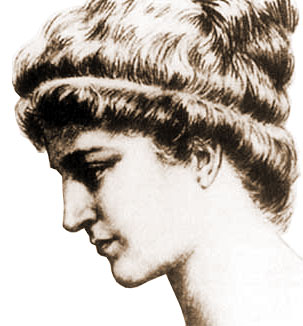
\includegraphics[width=0.12\textwidth]{Hypatia}

{\scriptsize Portrait imaginaire\par d'Hypatie d'Alexandrie\par}
}
\parbox{0.77\textwidth}{\begin{minipage}{0.65\textwidth}
\textbf{Hypatie d'Alexandrie} (vers 370 - 415)

Seule mathématicienne connue de l'Antiquité. Elle écrit notamment des commentaires sur l'arithmétique de Diophante et sur les tables de Ptolémée.
Elle meurt lapidée par des moines chrétiens fanatiques.
\end{minipage}}
\end{TP}

\begin{TP}[Chiffrement de Hill]

\partie{Partie A : Inverse de 23 modulo 26}
% {\color{H1}\textbf{Partie A : Inverse de 23 modulo 26}}
 
Soit l'équation :\enskip (E)~:\enskip  $23x - 26y = 1,$\enskip
où $x$ et $y$ désignent deux entiers relatifs.
\begin{enumerate}
\item Vérifier que le couple $(-9~;~-8)$ est solution de l'équation
  (E).
\item Résoudre alors l'équation (E). 
\item En déduire un entier $a$ tel que $0 \leqslant a \leqslant 25$ et $23a \equiv 1 \pmod {26}$.
\end{enumerate}

% {\color{H1}\textbf{Partie B : Codage et décodage}}
\partie{Codage et décodage}
 
Le chiffrement de Hill publié en 1929, est un chiffre polygraphique,
c'est-à-dire qu'on ne chiffre pas les lettres les unes après les
autres, mais par \ofg{paquets}. 

Voici un exemple \ofg{bigraphique},
c'est-à-dire où les lettres sont regroupées deux à deux.

\medskip
 
\begin{minipage}{0.8\textwidth}
\textbf{Étape 1} : On regroupe les lettres par 2. Chaque lettre est remplacée par un entier en utilisant le tableau ci-dessous :

\medskip
 
\begin{center}
\renewcommand*\tabularxcolumn[1]{>{\centering\arraybackslash}m{#1}}
{\footnotesize\begin{ttableau}{0.95\linewidth}{13}\hline
\rowcolor{FondTableaux}A& B& C& D& E& F& G& H& I& J& K& L& M\\ \hline
0& 1& 2& 3& 4& 5& 6& 7& 8& 9& 10& 11& 12\\ \hline \hline
\rowcolor{FondTableaux}N& O& P& Q& R& S& T& U& V& W& X& Y& Z\\ \hline
13& 14& 15& 16& 17& 18& 19& 20& 21& 22& 23& 24& 25\\ \hline
\end{ttableau}}
\end{center}


On obtient des couples d'entiers $\left(x_{1}~;~x_{2}\right)$ où
$x_{1}$ correspond à la première lettre et\\
$x_{2}$ correspond à la deuxième lettre.
 
\textbf{Étape 2} : Chaque couple $\left(x_{1}~;~x_{2}\right)$ est transformé en $\left(y_{1}~;~y_{2}\right)$ tel que :\vspace{-5pt}

$$\left(S_{1}\right)\enskip
\left\{\begin{aligned}
&y_{1} \equiv 11x_{1} + 3x_{2}~(26)\\ 
&y_{2} \equiv 	7x_{1} + 4x_{2}~(26)
\end{aligned}\right.
\quad  	\text{avec}\enskip 0\Inf y_{1}\Inf25\enskip\text{et}\enskip0 \Inf y_{2} \Inf25.\vspace{-5pt}$$

\textbf{Étape 3 :} Chaque couple $\left(y_{1}~;~y_{2}\right)$ est transformé en un couple de deux lettres en utilisant le tableau de correspondance donné dans l'étape 1. On regroupe ensuite les lettres.\medskip

Exemple : $\underbrace{\text{TE}}_{{\text{mot en
      clair}}}\stackrel{\text{étape } 1}{\Longrightarrow}   
(19,4) \stackrel{\text{étape}\ 2}{\Longrightarrow} (13,19)
\stackrel{\text{étape}\ 3}{\Longrightarrow}
\underbrace{\text{NT}}_{{\text{mot codé}}}$
\end{minipage}

\begin{enumerate}
\item Coder le mot ST. 
\item On décide de construire un algorithme permettant d'aller plus vite. 

On propose l'algorithme  à compléter suivant où E($x$) désigne la partie entière de $x$ :

\begin{center}
\begin{algorithme}
\BlocVariables
\DeclareVar{$X$, $Y$, $Z$, $T$}{\normalfont entiers}{}
\BlocEntrees
\Saisir{$X$, $Y$}
\BlocTraitements
\DonnerValeur{$Z$}{\dots}\vspace{3pt}%$11X+3Y$
\DonnerValeur{$T$}{\dots}\vspace{3pt}%$7X+4Y$
\DonnerValeur{$Z$}{\enskip$Z-26\times\text{\normalfont E}\left(\dfrac{Z}{26}\right)$}\vspace{3pt}
\DonnerValeur{$T$}{\enskip$T-26\times\text{\normalfont E}\left(\dfrac{T}{26}\right)$}
\BlocAffichage
\AfficherVarS{$Z$, $T$}
\end{algorithme}
\end{center}\medskip

\begin{enumerate}
\item Coder PALACE et RAPACE.
\item Que constatez-vous ?
\end{enumerate}

\item On veut maintenant déterminer la procédure de décodage.
\begin{enumerate}
\item Montrer que tout couple $\left(x_{1}~;~x_{2}\right)$ vérifiant
  les équations du système $\left(S_{1}\right)$ vérifie aussi les
  équations du système :\vspace{-5pt}
$$\left(S_{2}\right)\enskip
\left\{\begin{aligned}
&23x_{1} \equiv 4y_{1} + 23y_{2}~(26)\\ 
&23x_{2} \equiv 19y_{1} + 11y_{2}~(26)
\end{aligned}\right.$$

\item À l'aide de la partie A, montrer que tout couple
  $\left(x_{1}~;~x_{2}\right)$ vérifiant les équations du système
  $\left(S_{2}\right)$ vérifie aussi les équations du système
  :\vspace{-5pt}
$$\left(S_{3}\right)\enskip
\left\{\begin{aligned}
&x_{1} \equiv 16y_{1} + y_{2}~(26)\\
&x_{2} \equiv 11y_{1} + 5y_{2}~(26)
\end{aligned}\right.$$
  
\item Montrer que tout couple $\left(x_{1}~;~x_{2}\right)$ vérifiant
  les équations du système $\left(S_{3}\right)$ vérifie aussi les
  équations du système $\left(S_{1}\right)$.
\item Écrire un algorithme sur le même principe que l'algorithme de chiffrage pour décoder un mot.
\item Décoder le mot : PFXXKNU.
		
Ce mot étant de 7 lettres, ajouter la lettre W à la fin du mot pour avoir des paquets de deux lettres. Le décodage terminé, on supprimera la lettre dont le code est W. 
\end{enumerate}
\end{enumerate}
\end{TP}

